Este anexo apresenta os principais conceitos relacionados com a avaliação
da sustentabilidade segundo os fins do projeto SustenAgro, e como
foram usados no processo de avaliação de sustentabilidade.

\section{Sustentabilidade}

Não existe um consenso sobre a definição de sustentabilidade, mas
uma definição orientadora para os fins do presente projeto é a seguinte:
\begin{quotation}
``O desenvolvimento sustentável prevê o atendimento das necessidades
do presente sem comprometer a capacidade das gerações futuras de suprir
suas próprias necessidades, \foreignlanguage{english}{Brundtland Commission}''
\citep{Burton:1987,brundtland1987our}
\end{quotation}
Este conceito foi ratificado pela Conferência das Nações Unidas sobre
o Meio Ambiente e Desenvolvimento, a Rio-92 \citep{ehlers1996agricultura}
a Rio+20 \citep{ONU2012}, após do relatório \foreignlanguage{english}{Brundtland}
a ênfase do conceito desloca-se da integridade ambiental para o elemento
humano, gerando um equilíbrio entre as dimensões econômica, social
e ambiental \citep{van2005indicadores}.

\citet{gliessman2001agroecologia} teoriza que não há como alcançar
a sustentabilidade e, portanto, o seu conceito mais representativo,
pois a mesma permanece sempre no futuro, dado o compromisso que os
sistemas têm de garantir as necessidades das gerações futuras. Assim,
a sustentabilidade é algo relativo ao tempo, ou seja, um sistema pode
ser mais ou menos sustentável que outro dependendo do tempo em que
for avaliado e do entendimento da sustentabilidade neste contexto.

A sustentabilidade está vinculada a vários domínios de conhecimento,
um deles é a sustentabilidade em agricultura, que é de especial interesse
na segurança alimentar. segundo a FAO em 2050 a população mundial
atingirá 9.1 bilhões de pessoas \citep{fischer2009can}, o qual imporá
enormes desafios para garantir a sustentabilidade em meio do aumento
de alimentos. Por isso são necessários incentivos e políticas para
garantir a sustentabilidade na agricultura, através da geração de
estratégias que permitam conhecer o estado dos sistemas produtivos
e melhorar segundo as necessidades identificadas.

Segundo \citet{van2008integrated} os sistemas agrícolas evoluem continuamente
e são afetados por uma gama de forças globais e locais, sendo os tecnológicos
e políticos que mais influenciam na sustentabilidade da agricultura,
permitindo identificar e melhorar diversos aspectos da produção agrícola. 

Uma estratégia para quantificar a sustentabilidade é a definição métodos
e metodologias de avaliação, as quais utilizam indicadores. Um exemplo
deste enfoque é exposto por \citet{AlkanOlsson:2009} que desenvolveu
um \foreignlanguage{english}{\emph{framework}} de indicadores que
relaciona de uma maneira consistente as dimensões ambiental, econômica
e social do desenvolvimento sustentável, seu principal benefício é
uma relativa simplicidade na apresentação da informação e a possibilidade
de vincular os indicadores com objetivos políticos de cada dimensão
da sustentabilidade e assim facilitar a comparação dos impactos das
novas políticas em cada dimensão.

\section{Dimensões da Sustentabilidade}

As dimensões da sustentabilidade são classificações que permitem identificar
e agrupar conceitos de sustentabilidade\citep{AlkanOlsson:2009}.,
dependendo da teoria de sustentabilidade escolhida. Existem diversas
propostas de dimensões que podem ser usadas segundo a finalidade da
pesquisa. Um exemplo desta classificação é a assumida na pesquisa
de \citet{oliveira:2013} onde são definidas seis dimensões da sustentabilidade:
Ambiental, Social, Agrícola/Industrial, Produtos/Subprodutos, Tecnológica
e Política.

No caso do sistema SustenAgro determinou-se pela equipe de especialistas
em sustentabilidade fazer uma divisão segundo a proposta do Relatório
Brundtland \citep{brundtland1987our}, onde foram identificadas as
três dimensões da sustentabilidade: ambiental, social e econômica,
as quais têm a mesma importância gerando equilíbrio.

Ditas dimensões são sistemas complexos que integram fenômenos de natureza
diversa \citep{simon1991architecture}, integrando três subsistemas:
(i) o subsistema ambiental que fornece as condições físicas, químicas
e biológicas que suportam o desenvolvimento das culturas, (ii) o subsistema
social que integra organizações e pessoas que realizam a produção,
relacionando-se internamente e externamente com os sistemas produtivos
e (iii) o subsistema econômico que estabelece as condições de oferta
e demanda dos produtos e subprodutos do sistema de produção agrícola.
Das interações entre estes subsistemas, emerge um comportamento complexo
que requer uma abordagem holística e inter-relacionada para suportar
a tomada de decisões que garantam a sustentabilidade do sistema em
análise.

A Figura \ref{fig:sustainability_spheres} representa as três dimensões
com a sustentabilidade como a interseção entre elas.

\begin{figure}[h]
\begin{centering}
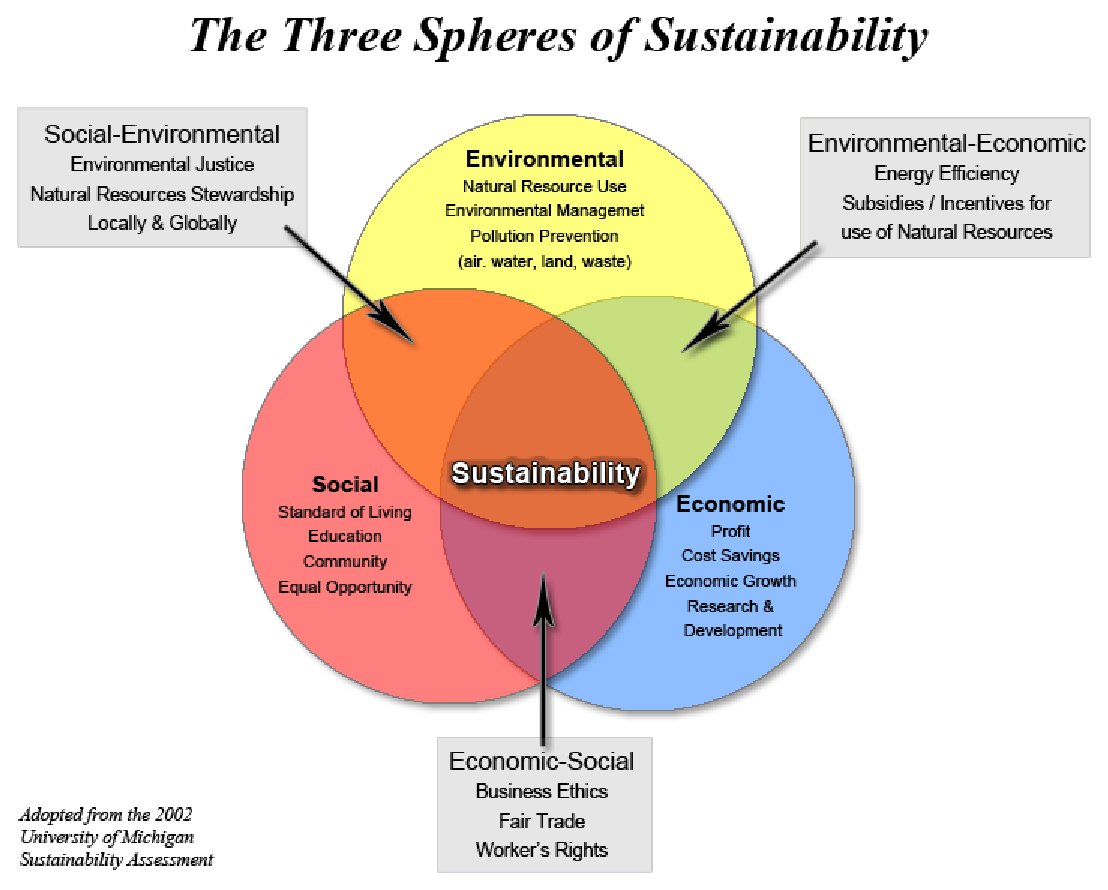
\includegraphics[width=1\columnwidth]{figures/sustainability_spheres}
\par\end{centering}
\caption{Dimensões da sustentabilidade \label{fig:sustainability_spheres}}
\end{figure}

\footnote{Tomada de: http://www.vanderbilt.edu/sustainvu/cms/files/sustainability\_spheres.png}Essas
dimensões serão usadas como contendedores gerais dos conceitos de
sustentabilidade em agricultura permitindo agrupar conceitos relacionados.

\section{Critérios de sustentabilidade}

São variáveis transversais quantitativas e qualitativas, que são monitoradas
regularmente para determinar os efeitos das atividades de intervenção
ou não-intervenção do sistema em avaliação \citep{deusdara2001criterios},
que estabelecem os preceitos de orientação para que os indicadores
sejam representativos para a sustentabilidade.

Cada indicador deverá atender pelo menos um dos critérios de sustentabilidade
para ser considerado um bom indicador de sustentabilidade. Os critérios
de sustentabilidade definidos pela equipe de especialistas são \citep{moura2002indicadores}:
\begin{itemize}
\item Produtividade: Relacionado a eficiência e custos.
\item Estabilidade: Capacidade do ecossistema de absorver perturbações e
permanecer inalterado (Comissão Econômica para a América Latina e
o Caribe/Programa das Nações Unidas para o Meio Ambiente, CEPAL\nomenclature{CEPAL}{Economic Commission for Latin America and the Caribbean}/PNUMA\nomenclature{PNUMA}{Programa das Nações Unidas para o Meio Ambiente},
1994) 
\item Equidade: Distribuição dos produtos do agroecossistema entre produtores
e consumidores (Dias Junior, 2000) 
\item Resiliência: Capacidade do ecossistema de retornar ao estado original
após de uma perturbação (CEPAL/PNUMA, 1994) 
\item Autonomia: Grau de integração do agroecossistema no fluxo de materiais,
energia e informação entre as partes constituintes e entre o agroecossistema
e o ambiente externo (Fernández, 1995)
\end{itemize}
Esses critérios guiam o desenvolvimento dos conceitos mais relevantes
das metodologias de avaliação de sustentabilidade, os indicadores,
e assim determinar instrumentos de medição que representem os aspectos
críticos do sistema em termos de sustentabilidade.

\section{Atributos Norteadores}

Embora a orientação para a elaboração de todas as variáveis relacionadas
a projetos de sustentabilidade devam atender pelo menos a três pilares:
ambiental, econômico, social, os atributos norteadores são formulados
para garantir as diretrizes no levantamento e validação dos indicadores,
e assim ter um modelo da sustentabilidade dos sistemas de produção
agrícola.

Após a agregação dos dados será possível visualizar as informações
disponíveis e eventuais lacunas para a sistematização dos componentes
dos sistemas produtivos em termos dos requisitos de sustentabilidade.
Em uma primeira instância, devem ser levantados dados referentes ao
solo, clima, água, ar, produção agroindustrial, divisas geradas, mão
de obra envolvida, empregos gerados, doações/benefícios indiretos
à sociedade, biodiversidade, etc.

Os atributos norteadores propostos para o sistema são:
\begin{itemize}
\item Dimensão Ambiental: solo, hídrico, clima, entre outros
\item Dimensão Social: saúde, capacitação, emprego, renda, entre outros
\item Dimensão Econômica: industrial, agrícola, produtividade, custo, entre
outros
\end{itemize}
Os atributos norteadores foram aplicados nos modelos do sistema SustenAgro
como contentores de indicadores os quais classificaram e relacionam
os indicadores em subgrupos das três dimensões da sustentabilidade,
permitindo desta maneira a organização e agrupamento do conhecimento
do domínio.

\section{Método SustenAgro}

O método SustenAgro foi construído a partir de literatura cientifica
e de contribuições de pesquisadores de instituições de pesquisa como
(IBGE\footnote{IBGE: \foreignlanguage{english}{Brazilian Institute of Geography and
Statistics}, \url{http://www.ibge.gov.br/home/}}, CONAB \footnote{CONAB: \foreignlanguage{english}{National Supply Company}, \url{http://www.conab.gov.br/}})
e validados por meio da técnica \foreignlanguage{english}{Delphi}
de consultas aos especialistas.

O método está composto pelos índices da eficiência e índice da sustentabilidade,
o índice da eficiência está composto por dois fatores de eficiência
tecnológica no campo e na indústria e o índice da sustentabilidade
está composto pelas dimensões ambientais, econômica e social.

A continuação serão apresentadas as fórmulas destes dois índices:

\subsection*{Índice de eficiência:}

As equações para calcular o índice da eficiência são:

\begin{algorithm}[h]
Fórmula de eficiência tecnologia no campo:

$efficiency(field)=\sum(CharacteristicsField*RelevanceProduction)*correctionFactor(0.8)$

Fórmula de eficiência tecnologia na indústria:

$efficiency(industry)=\sum(CharacteristicsProcessing*SugarcaneProcessing)*correctionFactor(0.2)$

Fórmula de eficiência produtiva e de custo:

$efficiencyAndCost=\sum(SugarcanEquality+\sum(Logistic+MarketVariables+Policies+Productivity))$

Índice de eficiência:

$EfficiencyIndex=\sum(efficiency(filed)+efficiency(industry))*efficiencyAndCost$

\caption{Fórmulas do índice de eficiência.}
\end{algorithm}


\subsection*{Índice de sustentabilidade}

As equações para calcular o índice de sustentabilidade são:

\begin{algorithm}[H]
Fórmula da dimensão ambiental:

$EnvironmentalIndex=\sum(EnvironmentalIndicator*EnvironmentIndicatorWeight)$

Fórmula da dimensão econômica:

$EconomicIndex=\sum(EconomicIndicator*EconomicIndicatorWeight)$

Fórmula da dimensão social:

$SocialIndex=\sum(SocialIndicator*SocialIndicatorWeight)$

Índice de sustentabilidade:

$SustainabilityIndex=\sum(EnvironmentalIndex+EconomicIndex+SocialIndex)/3$

\caption{Fórmulas do índice da sustentabilidade.}
\end{algorithm}

O usuário deverá ser informado da importância dos processos de avaliação,
exemplo dados pelos especialistas (não tem referências porque só são
exemplos): 
\begin{itemize}
\item “A crescente demanda de países desenvolvidos por produtos com garantia
de origem tem induzido aumento das certificações nas usinas no Brasil
(ALVES et al., 2008).” 
\item “A certificação tem sido uma importante forma de diferenciação de
commodities agrícolas, facilitando seu acesso aos mercados protegidos
dos países desenvolvidos.” 
\item “A caracterização climática, aliada aos detalhes de fertilidade e
manejo do solo (quantificação edafoclimática), são essenciais para
a determinação das regiões aptas ao cultivo de culturas de interesse
comercial (CIIAGRO, 2009).”
\end{itemize}
Depois de avaliar a sustentabilidade, o usuário receberá recomendações
classificadas sobre práticas de sustentabilidade recomendadas com
sua argumentação, exemplos (não tem referências) : 
\begin{itemize}
\item (Ambiental) “O sistema de plantio direto da cana-de-açúcar sobre leguminosas
proporciona maiores teores foliares de N e K na cana do que o plantio
convencional (JÚNIOR; COELHO, 2008)”.
\item (Ambiental) “Segundo Leme (2005), haveria redução de 36\% na emissão
de gases do efeito estufa (GEE) se a palha fosse queimada nas caldeiras
das usinas e destilarias, ao invés de ser queimada no campo”.
\item (Ambiental) “A queima da cana aumenta a erosão do solo e a poluição
do ar e reduz a qualidade da matéria-prima (LINS; SAAVEDR, 2007)”.
\item (Ambiental) “Quando não há queima da cana é comum, também, o aumento
do ataque de cigarrinhas, com perdas significativas de produção (ANDRADE;
DINIZ, 2007)”. 
\item (Econômico) “A utilização das colheitadeiras reverte-se em aumento
da produtividade e da qualidade da matéria-prima, bem como em diminuição
dos custos da produção agrícola, que representam entre 50\% e 60\%
em relação ao custo total (SCOPINHO, 1995)”.
\item (Econômico e Social) “A utilização das colheitadeiras em cooperativa
possibilita a soma das áreas de produtores próximos possibilitando
a mecanização em propriedades com restrição para mecanização”.
\item (Econômico) “Restrições físicas da propriedade (menos de 500 ha de
área com declividade inferior a 12\% e talhões menores que 800 metros)
dificultam a mecanização”. 
\end{itemize}

\section{Matriz de sustentabilidade}

Os índices de eficiência e de sustentabilidade quantificam a sustentabilidade
de uma unidade produtiva, e são representados por meio de uma matriz
que tem como finalidade relacionar o resultado da avaliação com determinadas
classificações correspondentes a cada uns dos quadrantes da matriz.
A figura \ref{fig:Matriz-de-sustentabilidade} representa cada uma
das classificações com os limiares correspondentes a cada índice.

\begin{figure}[H]
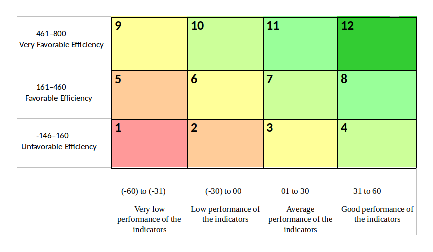
\includegraphics[width=0.8\columnwidth]{figures/SustaiabilityMatrixDesign}

\caption{Matriz de sustentabilidade \label{fig:Matriz-de-sustentabilidade}}

Matriz fornecida pelos pesquisadores da Embrapa Meio Ambiente.

\end{figure}


\section{Conclusões}

O método de avaliação de sustentabilidade foi validado pelos especialistas
e depois de varias iterações definiu-se uma versão estável, que foi
usada no desenvolvimento do Sistema SustenAgro, dito método é mantido
e atualizado pela Embrapa Meio Ambiente e os desenvolvedores de software
garantem que ele seja aplique corretamente mas não têm responsabilidade
nenhuma pela eficácia da aplicação dele.
